%%%%%%%%%%%%%%%%%%%%%%%%%%%%%%%%%%%%%%%%%%%%%%%%%%%%%%%%%%%
%				 _______ _    _  _____ 						
%				|__   __| |  | |/ ____|
%				   | |  | |__| | (___  
%				   | |  |  __  |\___ \ 
%				   | |  | |  | |____) |
%				   |_|  |_|  |_|_____/
%
%				 _               ____  
%				| |        /\   |  _ \ 
%				| |       /  \  | |_) |
%				| |      / /\ \ |  _ < 
%				| |____ / ____ \| |_) |
%				|______/_/    \_\____/ 
%
% _______ ______ __  __ _____  _            _______ ______ 
%|__   __|  ____|  \/  |  __ \| |        /\|__   __|  ____|
%   | |  | |__  | \  / | |__) | |       /  \  | |  | |__   
%   | |  |  __| | |\/| |  ___/| |      / /\ \ | |  |  __|  
%   | |  | |____| |  | | |    | |____ / ____ \| |  | |____ 
%   |_|  |______|_|  |_|_|    |______/_/    \_\_|  |______|
%
%%%%%%%%%%%%%%%%%%%%%%%%%%%%%%%%%%%%%%%%%%%%%%%%%%%%%%%%%%%
%%%%%%%%%%%%%%%%%%%%%%%%%%%%%%%%%%%%%%%%%%%%%%%%%%%%%%%%%%%
%%%%% DONT CHANGE ANYTHING BEFORE THE "TITLE" SECTION.%%%%%
%%%%%%%%%%%%%%%%%%%%%%%%%%%%%%%%%%%%%%%%%%%%%%%%%%%%%%%%%%%
%%%%%%%%%%%%%%%%%%%%%%%%%%%%%%%%%%%%%%%%%%%%%%%%%%%%%%%%%%%
\documentclass{article} % Don't change this
% _____        _____ _  __          _____ ______  _____ 
%|  __ \ /\   / ____| |/ /    /\   / ____|  ____|/ ____|
%| |__) /  \ | |    | ' /    /  \ | |  __| |__  | (___  
%|  ___/ /\ \| |    |  <    / /\ \| | |_ |  __|  \___ \ 
%| |  / ____ \ |____| . \  / ____ \ |__| | |____ ____) |
%|_| /_/    \_\_____|_|\_\/_/    \_\_____|______|_____/ 
%%%%%%%%%%%%%%%%%%%%%%%%%%%%%%%%%%%%%%%%%%%%%%%%%%%%%%%%

\usepackage[english]{babel}
\usepackage[utf8]{inputenc}
\usepackage[margin=1in]{geometry}
\usepackage{amsmath}
\usepackage{amsthm}
\usepackage{amsfonts}
\usepackage{amssymb}
\usepackage[usenames,dvipsnames]{xcolor}
\usepackage{graphicx}
\usepackage[siunitx]{circuitikz}
\usepackage{tikz}
\usepackage[colorinlistoftodos, color=orange!50]{todonotes}
\usepackage{hyperref}
\usepackage[numbers, square]{natbib}
\usepackage{fancybox}
\usepackage{epsfig}
\usepackage{soul}
\usepackage[framemethod=tikz]{mdframed}
\usepackage[font=small,labelfont=bf]{caption}


\usepackage{algorithm}
\usepackage[noend]{algpseudocode}

\usepackage[T1]{fontenc}
\usepackage[utf8]{inputenc}

%%%%%%%%%%%%%%%%%%%%%%%%%%%%%%%%%%%%%%%%%%%%%%%%%%%%%%%


%	  _____ _    _  _____ _______ ____  __  __ 
%	 / ____| |  | |/ ____|__   __/ __ \|  \/  |
%	| |    | |  | | (___    | | | |  | | \  / |
%	| |    | |  | |\___ \   | | | |  | | |\/| |
%	| |____| |__| |____) |  | | | |__| | |  | |
%	 \_____|\____/|_____/   |_|  \____/|_|  |_|
%%%%%%%%%%%%%%%%%%%%%%%%%%%%%%%%%%%%%%%%%%%%%%%%
%  _____ ____  __  __ __  __          _   _ _____   _____ 
% / ____/ __ \|  \/  |  \/  |   /\   | \ | |  __ \ / ____|
%| |   | |  | | \  / | \  / |  /  \  |  \| | |  | | (___  
%| |   | |  | | |\/| | |\/| | / /\ \ | . ` | |  | |\___ \ 
%| |___| |__| | |  | | |  | |/ ____ \| |\  | |__| |____) |
% \_____\____/|_|  |_|_|  |_/_/    \_\_| \_|_____/|_____/ 
%%%%%%%%%%%%%%%%%%%%%%%%%%%%%%%%%%%%%%%%%%%%%%%%%%%%%%%%%%

% SYNTAX FOR NEW COMMANDS:
%\newcommand{\new}{Old command or text}

% EXAMPLE:

\newcommand{\blah}{blah blah blah \dots}
\newcommand{\subf}[2]{%
  {\small\begin{tabular}[t]{@{}c@{}}
  #1\\#2
  \end{tabular}}%
}
%%%%%%%%%%%%%%%%%%%%%%%%%%%%%%%%%%%%%%%%%%%%%%%%%%%%%%%%%
%  _______ ______          _____ _    _ ______ _____  
% |__   __|  ____|   /\   / ____| |  | |  ____|  __ \ 
%    | |  | |__     /  \ | |    | |__| | |__  | |__) |
%    | |  |  __|   / /\ \| |    |  __  |  __| |  _  / 
%    | |  | |____ / ____ \ |____| |  | | |____| | \ \ 
%    |_|  |______/_/    \_\_____|_|  |_|______|_|  \_\
%%%%%%%%%%%%%%%%%%%%%%%%%%%%%%%%%%%%%%%%%%%%%%%%%%%%%%%%%
% \english
% \units 
% \spelling 
% \source 
% \concept
% \arbitrary{comment}{points}
% \summary{General Comments}

\setlength{\marginparwidth}{1cm}

% NEW COUNTERS
\newcounter{points}
\setcounter{points}{100}
\newcounter{spelling}
\newcounter{usage}
\newcounter{units}
\newcounter{other}
\newcounter{source}
\newcounter{concept}
\newcounter{missing}
\newcounter{math}

% COMMANDS
%\newcommand{\raisa}[2]{\colorbox{Yellow}{#1} \todo{#2}}
\newcommand{\arbitrary}[2]{\todo{#1 #2} \addtocounter{points}{#2} \addtocounter{other}{#2}}
\newcommand{\english}{\todo{LANGUAGE (-1)} \addtocounter{points}{-1}
\addtocounter{usage}{-1}}
\newcommand{\units}{\todo{UNITS (-1)} \addtocounter{points}{-1}
\addtocounter{units}{-1}}
\newcommand{\spelling}{\todo{SPELLING and GRAMMAR (-1)} \addtocounter{points}{-1}
\addtocounter{spelling}{-1}}
\newcommand{\source}{\todo{SOURCE(S) (-2)} \addtocounter{points}{-2}
\addtocounter{source}{-2}}
\newcommand{\concept}{\todo{CONCEPT (-2)} \addtocounter{points}{-2}
\addtocounter{concept}{-2}}
\newcommand{\missing}[2]{\todo{MISSING CONTENT (#1) #2} \addtocounter{points}{#1}
\addtocounter{missing}{#1}}
\newcommand{\maths}{\todo{MATH (-1)} \addtocounter{points}{-1}
\addtocounter{math}{-1}}

\newcommand{\summary}[1]{
\begin{mdframed}[nobreak=true]
\begin{minipage}{\textwidth}
\vspace{0.5cm}
\begin{center}
\Large{Grade Summary} \hrule 
\end{center} \vspace{0.5cm}
General Comments: #1

% \vspace{0.5cm}
Possible Points \dotfill 100 \\
Points Lost (Spelling and Grammar) \dotfill \thespelling \\
Points Lost (Language) \dotfill \theusage \\
Points Lost (Units) \dotfill \theunits \\
Points Lost (Math) \dotfill \themath \\
Points Lost (Sources) \dotfill \thesource \\
Points Lost (Concept) \dotfill \theconcept \\
Points Lost (Missing Content) \dotfill \themissing \\
Other \dotfill \theother \\[0.5cm]
\begin{center}
\large{\textbf{Grade:} \fbox{\thepoints}}
\end{center}
\end{minipage}
\end{mdframed}}

%#########################################################

%To use symbols for footnotes
\renewcommand*{\thefootnote}{\fnsymbol{footnote}}
%To change footnotes back to numbers uncomment the following line
%\renewcommand*{\thefootnote}{\arabic{footnote}}

% Enable this command to adjust line spacing for inline math equations.
% \everymath{\displaystyle}

% _______ _____ _______ _      ______ 
%|__   __|_   _|__   __| |    |  ____|
%   | |    | |    | |  | |    | |__   
%   | |    | |    | |  | |    |  __|  
%   | |   _| |_   | |  | |____| |____ 
%   |_|  |_____|  |_|  |______|______|
%%%%%%%%%%%%%%%%%%%%%%%%%%%%%%%%%%%%%%%

\title{
\normalfont \normalsize 
\textsc{Computational Neuroscience \\ 
IIT Madras} \\
[10pt] 
\rule{\linewidth}{0.5pt} \\[6pt] 
\huge Assignment 4 : Hopfield network \\
\rule{\linewidth}{2pt}  \\[10pt]
}
\author{Ganga Meghanath \\
EE15B025}

\begin{document}

\maketitle
% \noindent
% Date Performed \dotfill January 0, 0000 \\
% Partners \dotfill Full Name \\
% Instructor \dotfill Full Name \\

%%%%%%%%%%%%%%%%%%%%%%%%%%%%%%%%%%%%%%%

%			  ______      ____  
%			 |  ____/\   / __ \ 
%			 | |__ /  \ | |  | |
%			 |  __/ /\ \| |  | |
%			 | | / ____ \ |__| |
%			 |_|/_/    \_\___\_\
%%%%%%%%%%%%%%%%%%%%%%%%%%%%%%%%%%%%%%%%

%
% Ctrl + / to comment out a group of lines.
%
%
% LIST MORE COMMON COMMMANDS
% LIST USEFUL WEBSITES FOR TABLES, ETC
% WHAT TO DO WHEN YOUR CODE WONT COMPILE
% OVERLEAF SHORTCUTS
%



%%%%%%%%%%%%%%%%%%%%%%%%%%%%%%%%%%%%%%%


% _               ____  
%| |        /\   |  _ \ 
%| |       /  \  | |_) |
%| |      / /\ \ |  _ < 
%| |____ / ____ \| |_) |
%|______/_/    \_\____/ 
%%%%%%%%%%%%%%%%%%%%%%%%
%  _____ _______       _____ _______ _____ 
% / ____|__   __|/\   |  __ \__   __/ ____|
%| (___    | |  /  \  | |__) | | | | (___  
% \___ \   | | / /\ \ |  _  /  | |  \___ \ 
% ____) |  | |/ ____ \| | \ \  | |  ____) |
%|_____/   |_/_/    \_\_|  \_\ |_| |_____/ 
%%%%%%%%%%%%%%%%%%%%%%%%%%%%%%%%%%%%%%%%%%%
% _    _ ______ _____  ______ 
%| |  | |  ____|  __ \|  ____|
%| |__| | |__  | |__) | |__   
%|  __  |  __| |  _  /|  __|  
%| |  | | |____| | \ \| |____ 
%|_|  |_|______|_|  \_\______|
%%%%%%%%%%%%%%%%%%%%%%%%%%%%%%
\section{Aim}

\begin{itemize}
    \item Understand and Develop code for Hopfield Network for storing single and multiple patterns (images)
    \item Retrieve one of the stored patterns from the network corresponding to the input trigger
    \item Visualise the input triggers, original pattern and retrieved patterns
    \item Introduce noise into the strorage weights and analyse the effects on pattern retreival
\end{itemize}

%%%%%%%%%%%%%%%%%%%%%%%%%%%%%%%%%%%%%%%%%%%%%%%%%%%%%%%%%%%%%%%%%
\section{Preliminaries}
Since the given patterns are black and white (binary with 1 and -1), I have opted to use Discrete Hopfield Network over continuous since it's a simpler and direct implementation in such a scenario. \\

\noindent The patterns are stored in the weights matrix of the fully connected Hopfield Network as : $$\boldsymbol{W} = \frac{1}{N} \sum_i^{N_p} \boldsymbol{s}_i \boldsymbol{s}_i^T$$
where $\boldsymbol{W} \ \in \ \{ 1, -1\}^{N \times N}$, $\boldsymbol{s}_i \ \in \ \{ 1, -1\}^{N \times 1}$ denotes the $i^{th}$ pattern to be stored, $N_p$ denotes the total number of patterns to be stored in the network and $N$ denotes the total number of neurons in the network.\\

\noindent Note that all the patterns have been flattened out before storing it in the network and the all the patterns need to of the same dimension as that of the no. of neurons in the network. The weights from the $j^{th}$ neuron to the $i^{th}$ neuron is given by $\boldsymbol{W}[i][j]$.\\

\noindent The updates have been done in 2 different fashion :
\begin{itemize}
    \item[1] \textbf{Synchronous} updates : Here all the neurons are updated simultaneously at each iteration. Hence the current step update is made to all the neurons depending on the previous time step values of all the neurons. 
    \begin{equation}
        \boldsymbol{v}(t) = \sigma \big(\boldsymbol{W} \times \boldsymbol{v}(t-1) \big)
    \end{equation}
    where $\boldsymbol{v} \ \in \ \{ 1, -1\}^{N \times 1}$, $\boldsymbol{W} \ \in \ \{ 1, -1\}^{N \times N}$, t denotes the time step or iteration in this case and $\sigma$ denotes the sign function : \[
                    \sigma(x)= 
                            \begin{cases}
                                \frac{x}{|x|},& \text{if } x\neq 0\\
                                0,              & \text{otherwise}
                            \end{cases}
                \]
    \item[2] \textbf{Asynchronous} updates : Here one randomly selected neuron is updated at each iteration. Hence the current step update is made to a randomly selected neuron depending on the previous time step values of all the neurons. 
    \begin{equation}
        v_i(t) = \sigma \big(\boldsymbol{W[i, :]} \times \boldsymbol{v}(t-1) \big)
    \end{equation}
    where $\boldsymbol{v} \ \in \ \{ 1, -1\}^{N \times 1}$, $\boldsymbol{W} \ \in \ \{ 1, -1\}^{N \times N}$, $v_i$ denotes $i^{th}$ neuron, $\boldsymbol{W[i, :]} \ \in \{ 1, -1\}^{1 \times N}$ denotes $i^{th}$ row of $\boldsymbol{W}$, t denotes the time step or iteration in this case and $\sigma$ denotes the sign function : \[
                    \sigma(x)= 
                            \begin{cases}
                                \frac{x}{|x|},& \text{if } x\neq 0\\
                                0,              & \text{otherwise}
                            \end{cases}
                \]
\end{itemize}

\noindent For all the below experiments, the hyperparameters used are :
\begin{table}[H]
  \begin{center}
    \begin{tabular}{|c|c|c|c|} % <-- Alignments: 1st column left, 2nd middle and 3rd right, with vertical lines in between
    \hline
      \textbf{Method} & \textbf{No. of Iterations} & \textbf{No. of Neurons} \\
      \hline
      Synchronous Update & 5 & 9000 \\
      Asynchronous Update & 100000 & 9000\\
      \hline
    \end{tabular}
  \end{center}
\end{table}

The flattened input triggers are used to initialise $\boldsymbol{v}$. \\

\noindent In order to avoid ambiguity while reading from the image file and ensure all elements are from $\{-1, 0, 1\}$, corresponding text files have been saved for original images as well as image patches which are read from inorder to store the patterns in the Hopfield Network.
%%%%%%%%%%%%%%%%%%%%%%%%%%%%%%%%%%%%%%%%%%%%%%%%%%%%%%%%%%%%%%%%%
\section{Question 1}
%------------------------------------------------------
\subsection*{Image Visualization}
The visualised patterns are :
\begin{figure}[H]
\begin{tabular}{ccccc}

\includegraphics[width=0.3\linewidth]{images/ball.jpg}
&
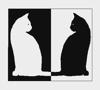
\includegraphics[width=0.3\linewidth]{images/cat.jpg}
&
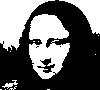
\includegraphics[width=0.3\linewidth]{images/mona.jpg}
\end{tabular}
\end{figure}

NOTE : The code for visualization can be found in \textit{``visualise.py''} \\\\
The code for Hopfield network with N=9000 neurons which are fully connected can be found in :
\begin{itemize}
    \item \textit{``Discrete/Single Pattern/hopfield$\_$ball.py''}
    \item \textit{``Discrete/Multiple Pattern/hopfield$\_$multi.py''} 
    \item \textit{``Discrete/Multiple Pattern/hopfiled$\_$weight$\_$noise.py''}
\end{itemize}


%%%%%%%%%%%%%%%%%%%%%%%%%%%%%%%%%%%%%%%%%%%%%%%%%%%%%%%%%%%%%%%%%
\section{Question 2}
%----------------------------------------------------------------
\subsection{Single pattern stored}
The image of the ball is saved in the network.\\\\
The code for Hofield Network can be found in \textit{``Discrete/Single Pattern/hopfield$\_$ball.py''}.

%----------------------------------------------------------------
\subsection{Input Trigger}
The input triggers are given by :
\begin{figure}[H]
\begin{tabular}{ccccc}

\includegraphics[width=0.22\linewidth]{images/ball_init1.jpg}
&

\includegraphics[width=0.22\linewidth]{images/ball_init2.jpg}
&

\includegraphics[width=0.22\linewidth]{images/ball_init3.jpg}
&

\includegraphics[width=0.22\linewidth]{images/ball_init4.jpg}
\end{tabular}
\end{figure}

\noindent NOTE : The code forgenerating the input triggers can be found in \textit{``Discrete/Single Pattern/generate$\_$patch.py.py''}
%----------------------------------------------------------------
\subsection{RMS Error and Pattern Retrieval}

\subsubsection{Synchronous Updates}
The corresponding RMS errors are given by :
\begin{figure}[H]
\begin{tabular}{ccccc}
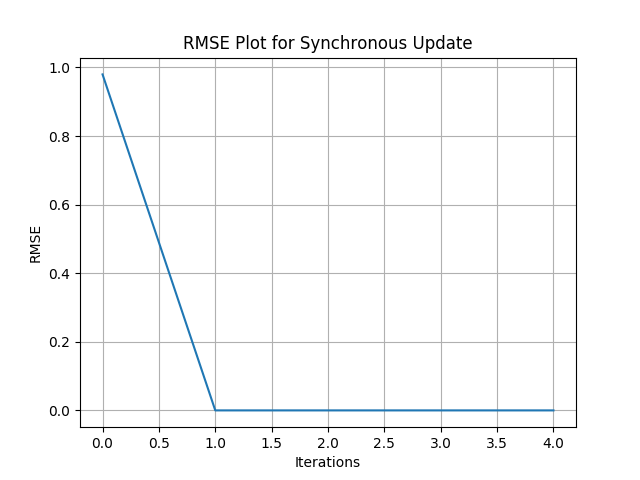
\includegraphics[width=0.22\linewidth]{images/Sync_Plot_1.png}
&
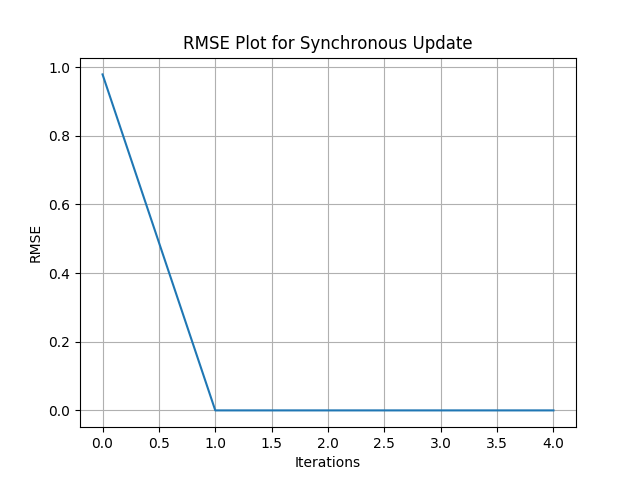
\includegraphics[width=0.22\linewidth]{images/Sync_Plot_2.png}
&
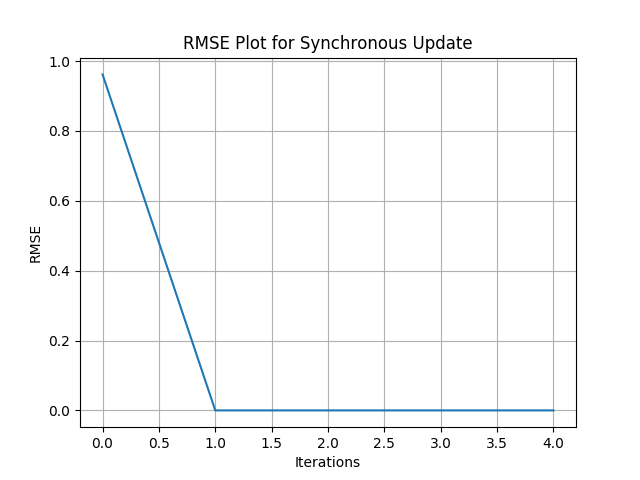
\includegraphics[width=0.22\linewidth]{images/Sync_Plot_3.png}
&
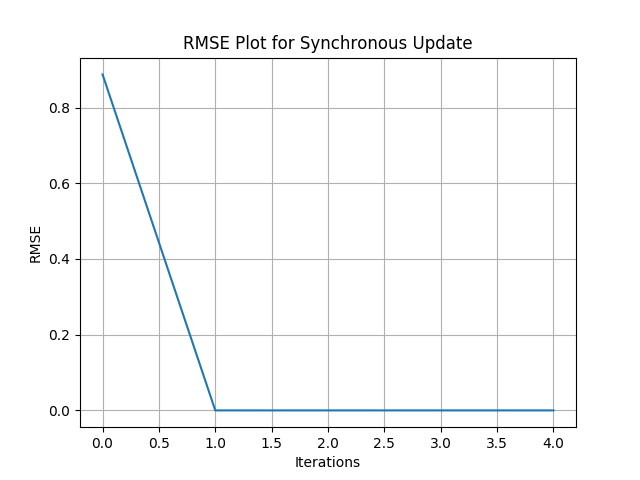
\includegraphics[width=0.22\linewidth]{images/Sync_Plot_4.png}
\end{tabular}
\end{figure}

\noindent The corresponding reconstructions are given by :
\begin{figure}[H]
\begin{tabular}{ccccc}

\includegraphics[width=0.22\linewidth]{images/Sync_ball_reconstruct_1.png}
&

\includegraphics[width=0.22\linewidth]{images/Sync_ball_reconstruct_2.png}
&

\includegraphics[width=0.22\linewidth]{images/Sync_ball_reconstruct_3.png}
&

\includegraphics[width=0.22\linewidth]{images/Sync_ball_reconstruct_4.png}
\end{tabular}
\end{figure}



\subsubsection{Asynchronous Updates}
The corresponding RMS errors are given by :
\begin{figure}[H]
\begin{tabular}{ccccc}
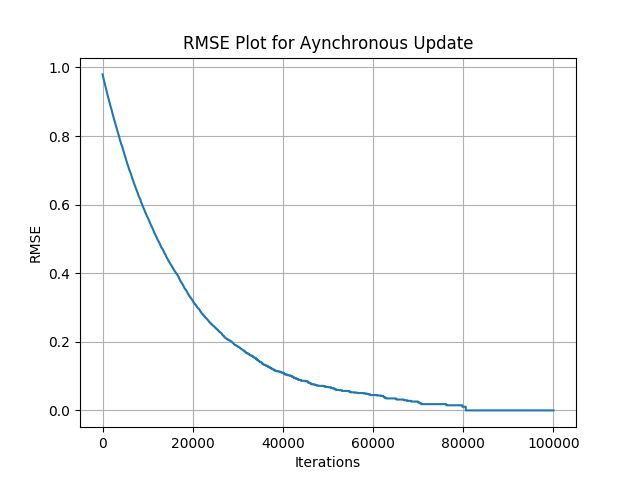
\includegraphics[width=0.22\linewidth]{images/Async_Plot_1.png}
&
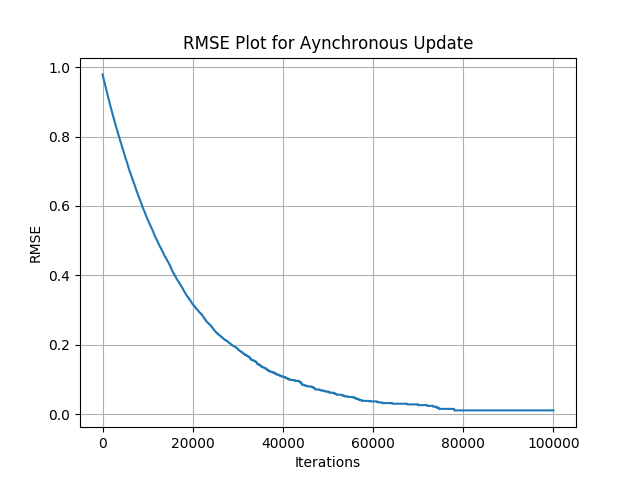
\includegraphics[width=0.22\linewidth]{images/Async_Plot_2.png}
&
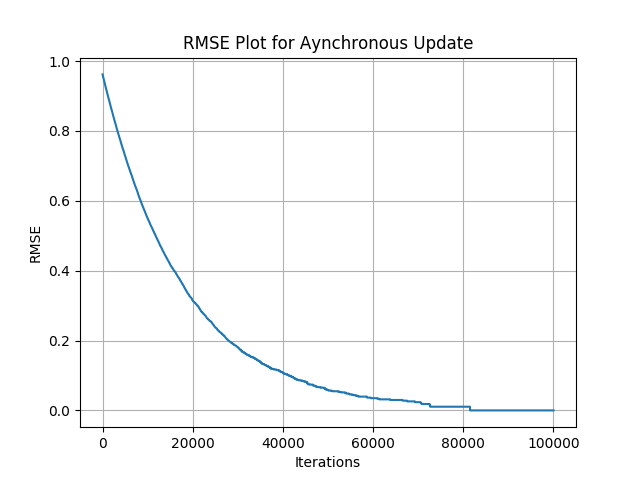
\includegraphics[width=0.22\linewidth]{images/Async_Plot_3.png}
&
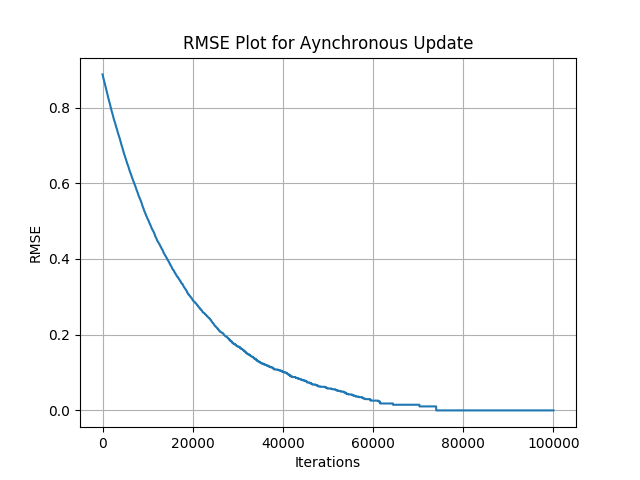
\includegraphics[width=0.22\linewidth]{images/Async_Plot_4.png}
\end{tabular}
\end{figure}

The corresponding reconstructions are given by :
\begin{figure}[H]
\begin{tabular}{ccccc}

\includegraphics[width=0.22\linewidth]{images/Async_ball_reconstruct_1.png}
&

\includegraphics[width=0.22\linewidth]{images/Async_ball_reconstruct_2.png}
&

\includegraphics[width=0.22\linewidth]{images/Async_ball_reconstruct_3.png}
&

\includegraphics[width=0.22\linewidth]{images/Async_ball_reconstruct_4.jpg}
\end{tabular}
\end{figure}

%%%%%%%%%%%%%%%%%%%%%%%%%%%%%%%%%%%%%%%%%%%%%%%%%%%%%%%%%%%%%%%%%
\section{Question 3}
%----------------------------------------------------------------
\subsection{Multiple patterns stored}
The image of the ball, cat and monalisa are saved in the network.\\\\
The code for Hofield Network can be found in \textit{``Discrete/Multiple Pattern/hopfield$\_$multi.py''}.

%----------------------------------------------------------------
\subsection{Input Trigger}
The input triggers for \textit{ball}, \textit{cat} and \textit{Monalisa} are given by :
\begin{figure}[H]
\begin{tabular}{ccccc}

\includegraphics[width=0.3\linewidth]{images/ball_init.jpg}
&

\includegraphics[width=0.3\linewidth]{images/cat_init.jpg}
&

\includegraphics[width=0.3\linewidth]{images/mona_init.jpg}
\end{tabular}
\end{figure}

\noindent NOTE : The code for generating the input triggers can be found in \textit{``Discrete/Multiple Pattern/generate$\_$patch.py''}.


%----------------------------------------------------------------
\subsection{RMS Error and Pattern Retrieval}

\subsubsection{Synchronous Updates}
The corresponding RMS errors are given by :
\begin{figure}[H]
\begin{tabular}{ccccc}
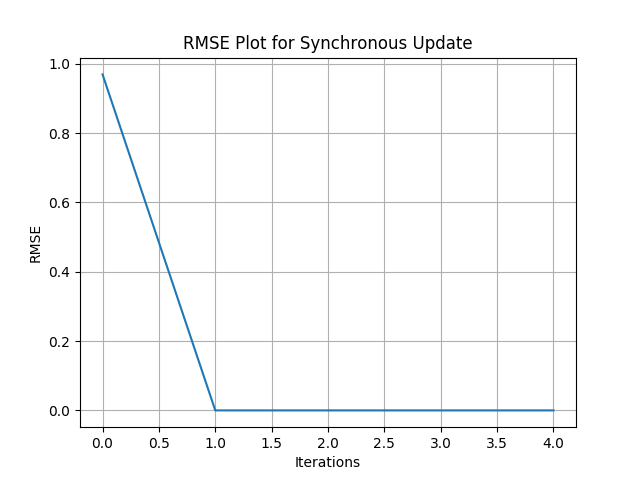
\includegraphics[width=0.3\linewidth]{images/Sync_Plot_ball.png}
&
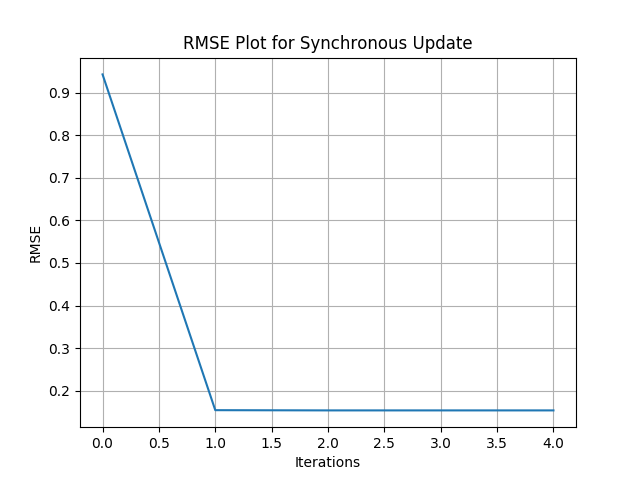
\includegraphics[width=0.3\linewidth]{images/Sync_Plot_cat.png}
&
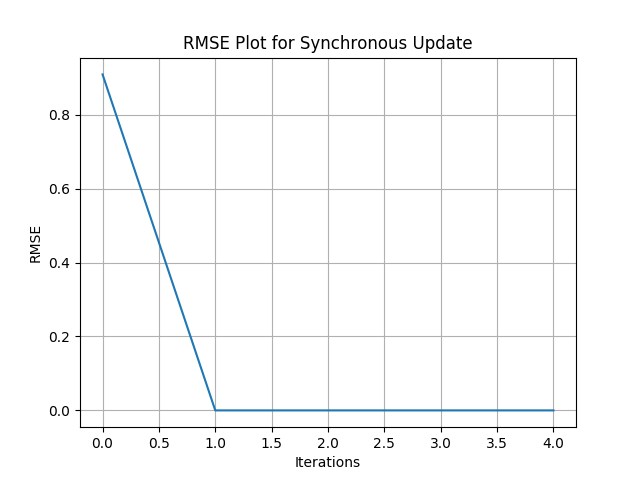
\includegraphics[width=0.3\linewidth]{images/Sync_Plot_mona.png}
\end{tabular}
\end{figure}


\noindent The corresponding reconstructions are given by :
\begin{figure}[H]
\begin{tabular}{ccccc}

\includegraphics[width=0.3\linewidth]{images/Sync_reconstruct_ball.png}
&

\includegraphics[width=0.3\linewidth]{images/Sync_reconstruct_cat.png}
&
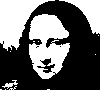
\includegraphics[width=0.3\linewidth]{images/Sync_reconstruct_mona.png}
\end{tabular}
\end{figure}




\subsubsection{Asynchronous Updates}
The corresponding RMS errors are given by :
\begin{figure}[H]
\begin{tabular}{ccccc}
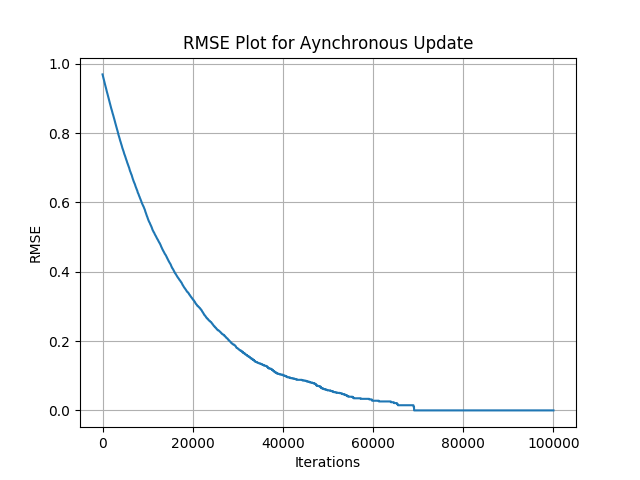
\includegraphics[width=0.3\linewidth]{images/Async_Plot_ball.png}
&
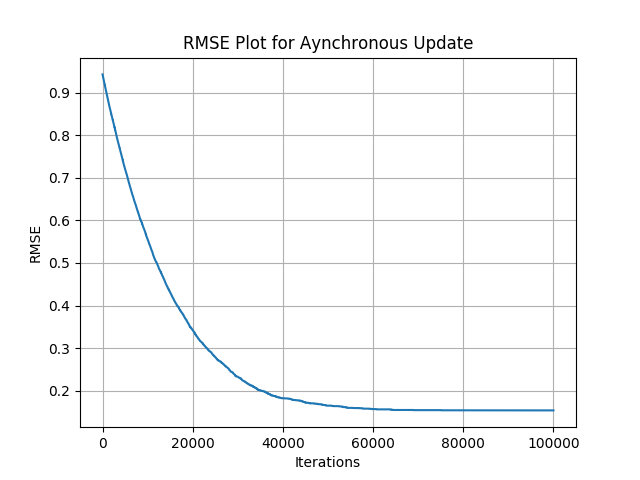
\includegraphics[width=0.3\linewidth]{images/Async_Plot_cat.png}
&
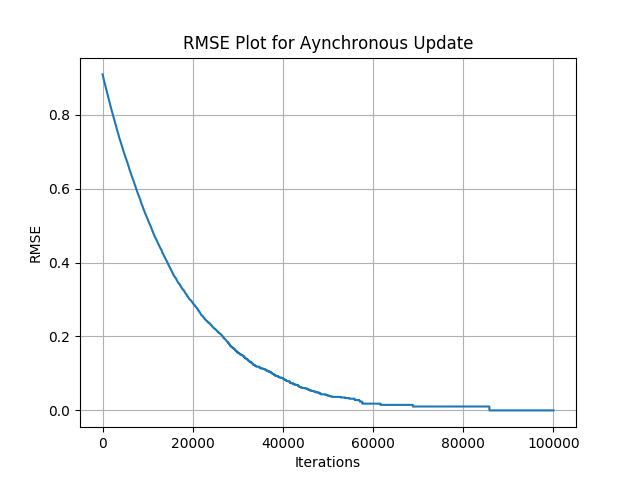
\includegraphics[width=0.3\linewidth]{images/Async_Plot_mona.png}
\end{tabular}
\end{figure}

\noindent The corresponding reconstructions are given by :
\begin{figure}[H]
\begin{tabular}{ccccc}

\includegraphics[width=0.3\linewidth]{images/Async_reconstruct_ball.png}
&

\includegraphics[width=0.3\linewidth]{images/Async_reconstruct_cat.png}
&
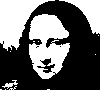
\includegraphics[width=0.3\linewidth]{images/Async_reconstruct_mona.png}
\end{tabular}
\end{figure}



%----------------------------------------------------------------
\subsection{Corrupting the weights that store the patterns}
X$\%$ of weights are made to be zero (randomly). \\\\
The input triggers for \textit{ball}, \textit{cat} and \textit{Monalisa}, used for the purpose are given by :
\begin{figure}[H]
\begin{tabular}{ccccc}

\includegraphics[width=0.3\linewidth]{images/ball_init_noise.jpg}
&

\includegraphics[width=0.3\linewidth]{images/cat_init_noise.jpg}
&

\includegraphics[width=0.3\linewidth]{images/mona_init_noise.jpg}
\end{tabular}
\end{figure}


\noindent NOTE : The code for generating the input triggers can be found in \textit{``Discrete/Multiple Pattern/generate$\_$patch.py''}.\\

\noindent For generation of random X$\%$ of noise, the following snippet has been utilised :
\begin{itemize}
    \item Consider $\boldsymbol{W} = \begin{bmatrix}
                                    1 & 1 & -1 \\
                                    -1 & -1 & -1\\
                                    -1 & 1 & 1 \\
                                    \end{bmatrix}$
    \item X$\_$val = int(X*N*N) gives no. of random $0$s to be generated. In this case $N=3$ and $X = 25\%$ gives X$\_$val = 2.
    \item mask = np.hstack(( np.ones((1, int(N*N-X$\_$val))) , np.zeros((1,X$\_$val)) )) gives :\\ $mask = \begin{bmatrix}
                                    1 & 1 & 1 &
                                    1 & 1 & 1 &
                                    1 & 0 & 0 
                                    \end{bmatrix}$ 
    \item mask = np.reshape(mask[0][np.random.permutation(N*N)], [N,N]) gives : 
                                    $mask = \begin{bmatrix}
                                                1 & 0 & 1 \\
                                                1 & 1 & 0\\
                                                1 & 1 & 1 \\
                                                \end{bmatrix}$
    \item W = W*mask (element-wise product) gives :  $\boldsymbol{W} = \begin{bmatrix}
                                                    1 & 0 & -1 \\
                                                    -1 & -1 & 0\\
                                                    -1 & 1 & 1 \\
                                                    \end{bmatrix}$
\end{itemize}
% +++++++++++++++++++++++++++++++++++++++++++++
\subsubsection{X = 25$\%$}

\textbf{Synchronous Updates}\\
The corresponding RMS errors are given by :
\begin{figure}[H]
\begin{tabular}{ccccc}
\includegraphics[width=0.3\linewidth]{images/Sync_Plot_ball_noise_25_0.png}
&
\includegraphics[width=0.3\linewidth]{images/Sync_Plot_cat_noise_25.png}
&
\includegraphics[width=0.3\linewidth]{images/Sync_Plot_mona_noise_25.png}
\end{tabular}
\end{figure}


\noindent The corresponding reconstructions are given by :
\begin{figure}[H]
\begin{tabular}{ccccc}
\includegraphics[width=0.3\linewidth]{images/Sync_reconstruct_ball_noise_25.png}
&
\includegraphics[width=0.3\linewidth]{images/Sync_reconstruct_cat_noise_25.png}
&
\includegraphics[width=0.3\linewidth]{images/Sync_reconstruct_mona_noise_25.png}
\end{tabular}
\end{figure}




\subsubsection{Asynchronous Updates}
The corresponding RMS errors are given by :
\begin{figure}[H]
\begin{tabular}{ccccc}
\includegraphics[width=0.3\linewidth]{images/Async_Plot_ball_noise_25_0.png}
&
\includegraphics[width=0.3\linewidth]{images/Async_Plot_cat_noise_25_0.png}
&
\includegraphics[width=0.3\linewidth]{images/Async_Plot_mona_noise_25_0.png}
\end{tabular}
\end{figure}

\noindent The corresponding reconstructions are given by :
\begin{figure}[H]
\begin{tabular}{ccccc}
\includegraphics[width=0.3\linewidth]{images/Async_reconstruct_ball_noise_25_0.png}
&
\includegraphics[width=0.3\linewidth]{images/Async_reconstruct_cat_noise_25_0.png}
&
\includegraphics[width=0.3\linewidth]{images/Async_reconstruct_mona_noise_25_0.png}
\end{tabular}
\end{figure}


% +++++++++++++++++++++++++++++++++++++++++++++
\subsubsection{X = 50$\%$}

\textbf{Synchronous Updates}\\
The corresponding RMS errors are given by :
\begin{figure}[H]
\begin{tabular}{ccccc}
\includegraphics[width=0.3\linewidth]{images/Sync_Plot_ball_noise_50_0.png}
&
\includegraphics[width=0.3\linewidth]{images/Sync_Plot_cat_noise_50.png}
&
\includegraphics[width=0.3\linewidth]{images/Sync_Plot_mona_noise_50.png}
\end{tabular}
\end{figure}


\noindent The corresponding reconstructions are given by :
\begin{figure}[H]
\begin{tabular}{ccccc}
\includegraphics[width=0.3\linewidth]{images/Sync_reconstruct_ball_noise_50.png}
&
\includegraphics[width=0.3\linewidth]{images/Sync_reconstruct_cat_noise_50.png}
&
\includegraphics[width=0.3\linewidth]{images/Sync_reconstruct_mona_noise_50.png}
\end{tabular}
\end{figure}




\subsubsection{Asynchronous Updates}
The corresponding RMS errors are given by :
\begin{figure}[H]
\begin{tabular}{ccccc}
\includegraphics[width=0.3\linewidth]{images/Async_Plot_ball_noise_50_0.png}
&
\includegraphics[width=0.3\linewidth]{images/Async_Plot_cat_noise_50_0.png}
&
\includegraphics[width=0.3\linewidth]{images/Async_Plot_mona_noise_50_0.png}
\end{tabular}
\end{figure}

\noindent The corresponding reconstructions are given by :
\begin{figure}[H]
\begin{tabular}{ccccc}
\includegraphics[width=0.3\linewidth]{images/Async_reconstruct_ball_noise_50_0.png}
&
\includegraphics[width=0.3\linewidth]{images/Async_reconstruct_cat_noise_50_0.png}
&
\includegraphics[width=0.3\linewidth]{images/Async_reconstruct_mona_noise_50_0.png}
\end{tabular}
\end{figure}


% +++++++++++++++++++++++++++++++++++++++++++++
\subsubsection{X = 80$\%$}

\textbf{Synchronous Updates}\\
The corresponding RMS errors are given by :
\begin{figure}[H]
\begin{tabular}{ccccc}
\includegraphics[width=0.3\linewidth]{images/Sync_Plot_ball_noise_80_0.png}
&
\includegraphics[width=0.3\linewidth]{images/Sync_Plot_cat_noise_80.png}
&
\includegraphics[width=0.3\linewidth]{images/Sync_Plot_mona_noise_80.png}
\end{tabular}
\end{figure}


\noindent The corresponding reconstructions are given by :
\begin{figure}[H]
\begin{tabular}{ccccc}
\includegraphics[width=0.3\linewidth]{images/Sync_reconstruct_ball_noise_80.png}
&
\includegraphics[width=0.3\linewidth]{images/Sync_reconstruct_cat_noise_80.png}
&
\includegraphics[width=0.3\linewidth]{images/Sync_reconstruct_mona_noise_80.png}
\end{tabular}
\end{figure}




\subsubsection{Asynchronous Updates}
The corresponding RMS errors are given by :
\begin{figure}[H]
\begin{tabular}{ccccc}
\includegraphics[width=0.3\linewidth]{images/Async_Plot_ball_noise_80_0.png}
&
\includegraphics[width=0.3\linewidth]{images/Async_Plot_cat_noise_80_0.png}
&
\includegraphics[width=0.3\linewidth]{images/Async_Plot_mona_noise_80_0.png}
\end{tabular}
\end{figure}

\noindent The corresponding reconstructions are given by :
\begin{figure}[H]
\begin{tabular}{ccccc}
\includegraphics[width=0.3\linewidth]{images/Async_reconstruct_ball_noise_80_0.png}
&
\includegraphics[width=0.3\linewidth]{images/Async_reconstruct_cat_noise_80_0.png}
&
\includegraphics[width=0.3\linewidth]{images/Async_reconstruct_mona_noise_80_0.png}
\end{tabular}
\end{figure}

\end{document} % NOTHING AFTER THIS LINE IS PART OF THE DOCUMENT
 ______ ______ ______ ______ ______ ______ ______ 
|______|______|______|______|______|______|______|
				  _____  ____  
				 / ____|/ __ \ 
				| |  __  |  | |
				| | |_ | |  | |
				| |__| | |__| |
				 \_____|\____/ 
 
 _    _  ____  _____  _   _ ______ _______ _____ _ 
| |  | |/ __ \|  __ \| \ | |  ____|__   __/ ____| |
| |__| | |  | | |__) |  \| | |__     | | | (___ | |
|  __  | |  | |  _  /| . ` |  __|    | |  \___ \| |
| |  | | |__| | | \ \| |\  | |____   | |  ____) |_|
|_|  |_|\____/|_|  \_\_| \_|______|  |_| |_____/(_)

 ______ ______ ______ ______ ______ ______ ______ 
|______|______|______|______|______|______|______|
